\documentclass{beamer}

\usetheme{Padova}

\title{Esame di Laurea in Informatica}
\subtitle{Implementazione di modelli di programmazione matematica per problemi di bin packing}
\author{Daniel Rossi}
\date{18 Dicembre 2018}


\begin{document}

\maketitle

%\begin{frame}{Outline}
%	\tableofcontents
%\end{frame}

\section{Introduzione}

\begin{frame}{Introduzione}
	\begin{minipage}[c]{0.45\textwidth}
		\large{\uppercase{Software supporto decisionale}}
	\end{minipage}
	\hfill
	\begin{minipage}[c]{0.45\textwidth}
		
\includegraphics[width=1\linewidth]{figures/logo-transcel}
	\end{minipage}
	\vspace{1.0em}
	\begin{itemize}
		\item agevolazione degli operatori;
		\item operatori meno esperti;
		\item aumento della produttivit\`a;
		\item informazioni sullo stato dei trasporti;
		\item stima di costi e profitti.
	\end{itemize}
\end{frame}

\begin{frame}{Introduzione}
	L'azienda ha sviluppato un'euristica per l'ottimizzazione dello spazio occupato dalle merci nel container del camion.
	\begin{figure}[H]
		\begin{center} 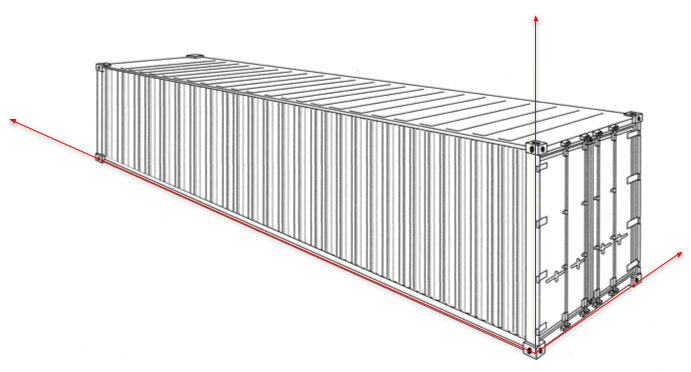
\includegraphics[width=1\linewidth]{figures/container_arrows}
		\end{center}
	\end{figure}
\end{frame}

\section{Proposta di stage}

\begin{frame}{Proposta di stage}
	\begin{alertblock}{Scopo}
		Lo scopo dello stage \`e  quello di realizzare dei modelli di programmazione lineare per la risoluzione dello \\ \textbf{Strip Packing Problem} da usare per valutare l'euristica aziendale
	\end{alertblock}
	\begin{itemize}
		\item \textbf{2D}: versione 2D;
		\item \textbf{2DR}: versione 2D con rotazione;
		\item \textbf{2DRS}: versione 2D con rotazione e sequenza di scarico;
		\item \textbf{3D}: versione 3D con rotazione e sovrapposizione.
	\end{itemize}
\end{frame}

\section{Modelli matematici}
\begin{frame}{Modello matematico}
	\begin{center}
		\begin{align*}
			& \underset{}{\text{min D}} \\
			  & \text{s.t.} &   & l_{ij} + l_{ji} + b_{ij} + b_{ji} \geq 1      & i < j    &   & i,j \in I \\
			  &             &   & y_i - y_j + M_d b_{ij} \leq M_d - d_i         &          &   & i,j \in I \\
			  &             &   & x_i - x_j + M_w l_{ij} \leq M_w - w_i         &          &   & i,j \in I \\
			  &             &   & x_i + w_i \leq W                              &          &   & i \in I   \\
			  &             &   & y_i + d_i \leq D                              &          &   & i \in I   \\
			  &             &   & b_{ij}, l_{ij} \in \{0,1\}                    & i \neq j &   & i,j \in I \\
			  &             &   & x_{i}, y_{i}, w_{i}, d_{i} \in \mathbb{R}^{+} &          &   & i \in I   
		\end{align*}
	\end{center}
		
\end{frame}

\section{Packing Problem}
\begin{frame}{Bin Packing Problem}
	\begin{block}{Insieme $I$}
		Si consideri un insieme $I = \{1,\dots,n\}$ di oggetti aventi dimensioni $w_{i}$, $d_{i}$ e $h_{i}$ con $i \in I$	
	\end{block}
	\begin{block}{insieme $J$}
		Si consideri un insieme $J = \{1,\dots,m\}$ di contenitori di uguale dimensione $W$, $D$ e $H$.
	\end{block}
	Diamo per ipotesi $w_{i} \leq W$, $d_{i} \leq D$ e $h_{i} \leq H$.
	\begin{alertblock}{Obiettivo}
		Minimizzare il numero di contenitori $J$ che riescano a contenere tutti gli oggetti dell'insieme $I$.
	\end{alertblock}
\end{frame}

\begin{frame}{Strip Packing Problem}
	Differenze dal precedente problema:\vspace{.5em}
	\begin{itemize}
		\item \textbf{Numero di contenitori}: singolo contenitore;
		\item \textbf{Dimensioni}: profondit\`a infinita;
	\end{itemize}
	\begin{alertblock}{Obiettivo}
		Minimizzare i metri lineari occupati rispetto la profondit\`a del contenitore.
	\end{alertblock}
\end{frame}

\begin{frame}{Sistema di riferimento}
	Convenzioni adottate: \vspace{.5em}
	\begin{center}
		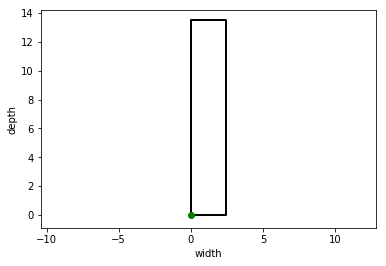
\includegraphics[width=9cm]{figures/cartesian_wd}
	\end{center}
\end{frame}

\begin{frame}{Elenco modelli}
	\begin{minipage}[c]{0.45\textwidth}
		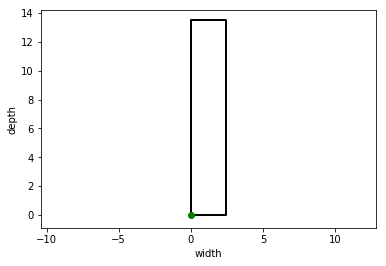
\includegraphics[width=\textwidth]{figures/cartesian_wd}
	\end{minipage}
	\hfill
	\begin{minipage}[c]{0.45\textwidth}
		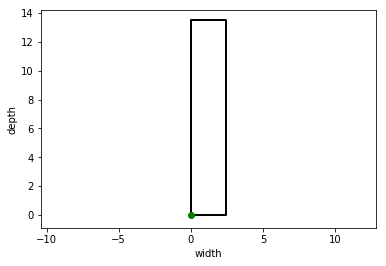
\includegraphics[width=\textwidth]{figures/cartesian_wd}
	\end{minipage}
	\begin{minipage}[c]{0.45\textwidth}
		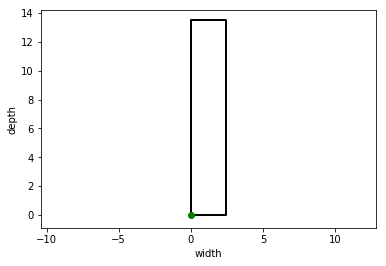
\includegraphics[width=\textwidth]{figures/cartesian_wd}
	\end{minipage}
	\hfill
	\begin{minipage}[c]{0.45\textwidth}
		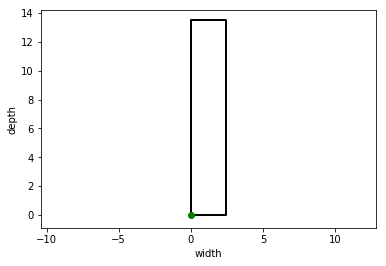
\includegraphics[width=\textwidth]{figures/cartesian_wd}
	\end{minipage}
\end{frame}

\begin{frame}{Modello 2D e 2DR}
												
	\begin{minipage}[c]{0.45\textwidth}
		\begin{alertblock}{Modello 2D}
			Limiti delle soluzioni
		\end{alertblock}	
	\end{minipage}
	\hfill
	\begin{minipage}[c]{0.45\textwidth}
		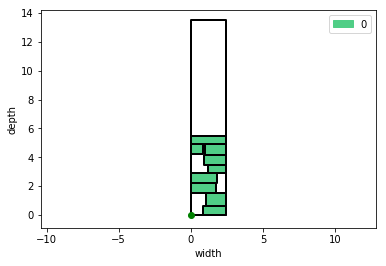
\includegraphics[width=1\linewidth]{figures/general2D}
	\end{minipage}
							
	\begin{minipage}[c]{0.45\textwidth}
		\begin{alertblock}{Modello 2DR}
			Ottimalit\`a della soluzione
		\end{alertblock}	
	\end{minipage}
	\hfill
	\begin{minipage}[c]{0.45\textwidth}
		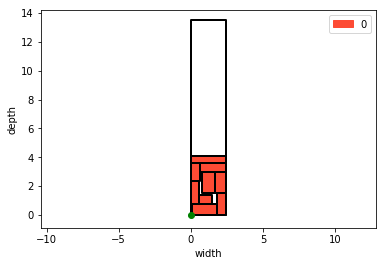
\includegraphics[width=1\linewidth]{figures/general2DR}
	\end{minipage}
\end{frame}

\begin{frame}{Modello 2DRS}
												
	\begin{minipage}[c]{0.45\textwidth}
		\begin{alertblock}{Vie di scarico}
			Deve essere presente almeno una via di scarico per ciascun pacco
		\end{alertblock}	
	\end{minipage}
	\hfill
	\begin{minipage}[c]{0.45\textwidth}
		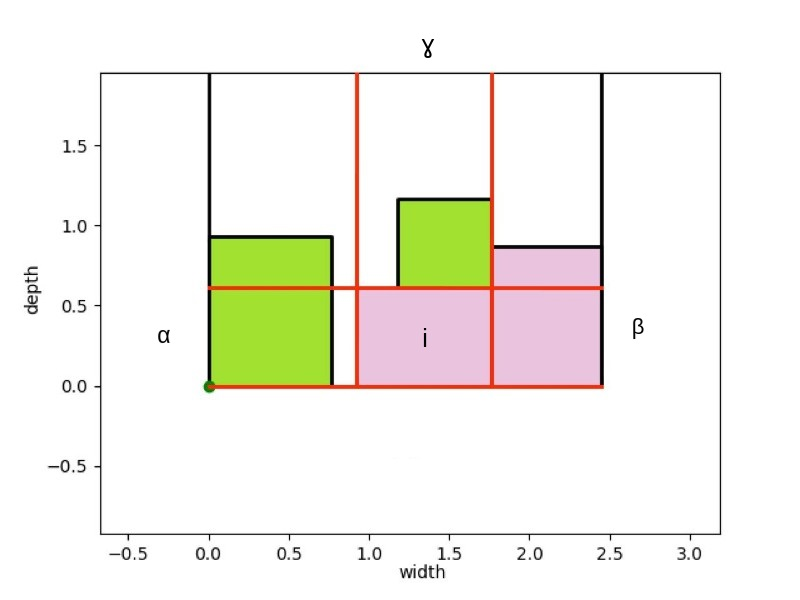
\includegraphics[width=1\linewidth]{figures/abg_2drs}
	\end{minipage}
							
	\begin{minipage}[c]{0.45\textwidth}
		\begin{alertblock}{Stabilit\`a generale}
			Le soluzione del modello non implementano la stabilit\`a generale
		\end{alertblock}	
	\end{minipage}
	\hfill
	\begin{minipage}[c]{0.45\textwidth}
		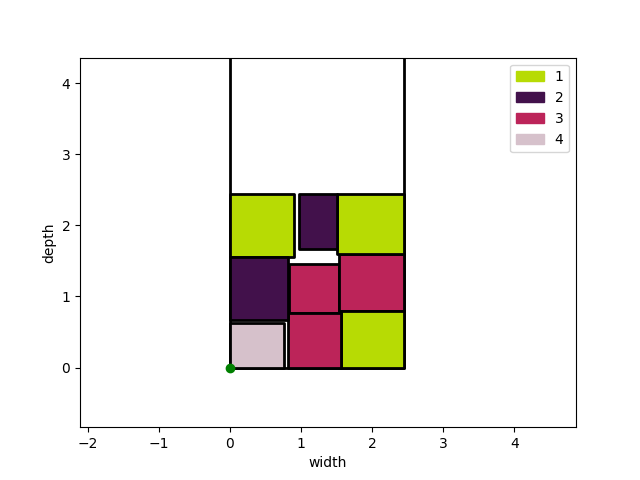
\includegraphics[width=1\linewidth]{figures/2d3d}
	\end{minipage}
\end{frame}

\begin{frame}{Modello 3D}
	\begin{minipage}[c]{0.45\textwidth}
		\begin{alertblock}{Stabilit\`a degli oggetti}
			Garantita sovrapponendo solo un oggetto
		\end{alertblock}	
	\end{minipage}
	\hfill
	\begin{minipage}[c]{0.45\textwidth}
		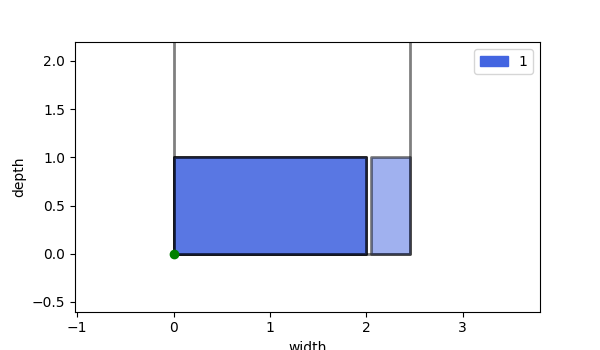
\includegraphics[width=1\linewidth]{figures/3dg}
	\end{minipage}
							
	\begin{minipage}[c]{0.45\textwidth}
		\begin{alertblock}{Oggetti stackable}
			In generale nei test non tutti gli oggetti erano sovrapponibili
		\end{alertblock}	
	\end{minipage}
	\hfill
	\begin{minipage}[c]{0.45\textwidth}
		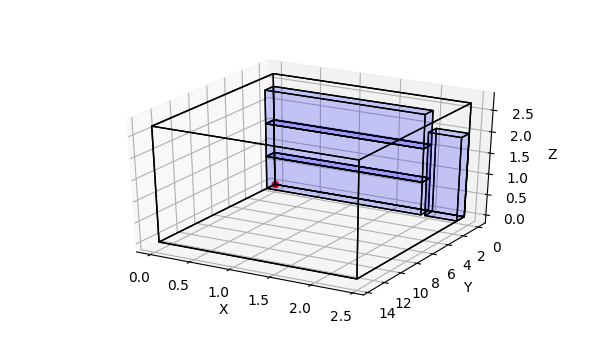
\includegraphics[width=1\linewidth]{figures/3d}
	\end{minipage}
\end{frame}

\begin{frame}{Errori confronto}
	\begin{block}{Objective value}
		Metri lineari minimizzati dal modello e dall'euristica:
		\begin{itemize}
			\item Objective modello: $Obj_m$
			\item Objective euristica: $Obj_h$
		\end{itemize}
	\end{block}
	\begin{minipage}[c]{0.45\textwidth}
		\begin{alertblock}{Errore assoluto:}
			$$\epsilon_a = Obj_h - Obj_m$$
		\end{alertblock}
	\end{minipage}
	\hfill
	\begin{minipage}[c]{0.45\textwidth}
		\begin{alertblock}{Errore relativo:}
			$$\epsilon_r = \frac{\epsilon_a}{Obj_m} \cdot 100$$
		\end{alertblock}	
	\end{minipage}
					
\end{frame}
					
\end{document}
